In this section, I will describe theoretical concepts: Tor network, Onion service,
Cryptocurrency, Dark marketplace.

% Tor network
\subsection{Tor network}
Tor is the second generation of onion routing system that addresses shortcomings
in the original design by adding perfect forward secrecy, congestion control,
directory servers, integrity checking, configurable exit policies, and a
practical design for location-hidden services through rendzvous points
~\cite{paper:tor_design}. Tor is a low-latency network system, which means that
the period of delaying is negligible for most users~\cite{report:overview_tor}.
This advantage makes Tor as a
suitable design for interactive tasks like web browsing or \acrshort{ssh}
connections~\cite{dis:usage_of_onion_services}. In addtion to the fast performance,
Tor communication service also provides the high degree of anonymity and privacy
in transferring network packets. Hence, Tor browser, a Firefox-based web browser
under Tor network, is widely used by activists and journalists for untraceable
communication~\cite{dis:usage_of_onion_services}. Moreover, ordinary citizens who have concerned their privacy during
Internet surfing select Tor-based applications as safe guards in the ungovernable
Internet environment.

The Tor users are protected by the common method of Internet surveillance, traffic
analysis. The source and destination of Internet communication can be exposed by
traffic analysis. These information reveal users' behaviour and interest~\cite{web:onion_network}.
To reduce the risk of traffic analysis, Tor distribute the connection between the
client and the final point over the chain of 3 Tor nodes, called \emph{relays}.
The circuit of encrypted connection over relays is described as the following steps.
% How does Tor anonymously route packets
\begin{enumerate}
    \item The Tor user obtains a list of Tor nodes from a
    directory server. Then public keys of selected relays are used to encrypt and
    encapsulate the network packet.  
    \item The Tor client connects to the guard relay, the first relay in the circuit
    of three Tor nodes. The encapsulated message is delivered to the guard relay.
    \item The guard relay decrypts the packet, using its private key, 
    and forward to the second node, the middle relay.
    \item The second node continues decrypting, using its private key, and then
    forwarding the message to the third node, the exit relay.
    \item The exit relay decrypts, using its private key, and forward the packet
    to the final destination, e.g, a web server.
\end{enumerate}

As shown in the aforementioned steps, a specific Tor relay only knows about the previous
sender and the next recipient. For example, the guard relay only learns about the Tor client
and the second hop, but not the final recipient. Thus, a complete path from the original
sender to the final destination is not exposed.

At each hop, the packet is decapsulated and decrypted by using private key of each relay,
``peeling off'' each encryption layer. It is similar to layers of onion and that is also
the reason why it is called \emph{onion routing}.

Although the traffic correlation attack is unavoidable in any low-latency anonymity
network, it is challenging to perform global traffic analysis due to the huge amount
of Tor users~\cite{dis:anonymity_system,paper:tor_design}. In addition to traffic and
time analysis, there are other techniques that reveal real identity of Tor users
~\cite{paper:de_tor}.

There are several types of routers, or relays, in the Tor network and soem of them
are aforementioned, including guard, middle, and exit. Since the exit relay communicates
publicly, outside the Tor network, to the destination, the IP address of it is exposed.
Moreover, the sender can also know the IP address of the first relay in the circuit of
three Tor routers.
By blocklisting the IP addresses of theses publicly known relays, many governments block
connections from their citizens to the Tor network. To address this problem, the bridge
node which is not listed in the public Tor directory is introduced. Thus, it is difficult
to block an IP address if it is not publicly known. However, several countries have
found means to detect and block connections to Tor bridges. Pluggable transport, a
special kind of bridge, is discovered address this problem by adding an extra layer
of obfuscation~\cite{web:relay_types}. According to \url{https://metrics.torproject.org},
in 2021, there are around 7000 relays and more than 2000 bridges running in the Tor
network.

Tor enables TCP-based applications to acquire online anonymity without modification
~\cite{paper:tor_design}. One of the popular Tor application is Tor browser. It is
a modified version of Mozilla Firefox Extended Support Release (ESR) with most-strict
security settings, such as NoScript and HTTPS Everywhere. This browser routes all
traffic through the Tor network and removes all possible fingerprinting methods,
including forging information about the operating system and hardwares
~\cite{dis:usage_of_onion_services}.
Furthermore, Tor Browser does not save sensitive data, including browsing history,
cache and cookies~\cite{dis:usage_of_onion_services}.

% Onion services
\subsection{Onion service}
%
Onion services, Tor hidden services, are an overlay network on top of TCP/IP;
thus, IP addresses are not used in the protocol~\cite{web:onion_service}. The
location and real IP address of Onion Service are protected, hidden from the
user. These hidden services are only available through the Tor network~\cite{paper:tor_design}.
Instead of IP address, onion service is indentified by the \emph{identity public key}.
This onion address which is in the form of \emph{x.onion} whose the first part \emph{x} is
the hash of public key of onion service, e.g, {\scriptsize \textbf{
database6e2t4yvdsrbw3qq6votzyfzspaso7sjga2tchx6tov23nsid.onion}}~\cite{dis:usage_of_onion_services}.

The onion service hides and protects itself by only allowing direct connections
from three pre-selected Tor relays, \emph{introduction points}. Every Tor client
and intermediary points have to be introduced by the three-hop circuit to reach
the onion service.
To be noticeable to clients, instead of using \gls{dns}, \gls{dht} is utilized
to match a onion service to its corresponding introduction points.

The onion service protocol is summarized in the following steps~\cite{paper:tor_design}.
\begin{enumerate}
    \item The onion service selects three Tor relays acting as its introduction
    points to build an anonymized circuit.
    \item The onion service generates a \emph{descriptor}, containing a list of
    introduction points, and signs this descriptor with the \emph{identity private
    key}. The key used to signing is the private part of the identity public key
    which is encoded in the onion service address.
    \item Given the onion address, the client requests the signed descriptor from
    from the \acrshort{dht}. Next, the client verify the signature of returned
    descriptor with the public key that is encoded in the onion address.
    \item The client randomly selects a Tor relay acting as a rendezvous point,
    build anonymized, three-hop circuit to it and send it an one-time secret.
    \item The generated one-time secret and the address of the rendezvous point
    are encrypted with the public key of the onion service and delivered to one of
    the introduction points through a anonymized circuit.
    \item The onion service decrypts and retrieve the rendezvous point and one-time
    secret. It connects and sends the one-time secret to the rendezvous point via
    a three-hop circuit.
    \item A complete circuit between the client and the onion service is built.
    It contains total five Tor relays, two from the client to the rendezvous point
    and three from the rendezvous point to the onion service. 
\end{enumerate}

The onion service protocol provides both end-to-end encryption and authentication
~\cite{web:onion_service}. Hence, it is impossible to censor onion services
and \gls{mitm} attack is prevented~\cite{dis:usage_of_onion_services}. As onion service
can publish contents anonymously, some of them are the sources of adverse content,
including illegal traded products, images of child abusing, etc~\cite{dis:usage_of_onion_services}.
However, many onion services
share content supporting human rights, meaningful for journalism and publishing
content that is censored by oppressive governments~\cite{dis:usage_of_onion_services}. 

\begin{figure}
    \centering
    
\includegraphics[width=\textwidth,height=\textheight,keepaspectratio]
    {screenshots/bbc_onion.png}
    \caption{Onion service mirroring BBC news website on Tor network.}
    \label{fig:onion_service}
\end{figure}

% Monetary system
\subsection{Cryptocurrency}
%
Onion service provides location hiding capacity and anonymity in content publishing
for illegal markeplaces. However, they also need a payment system that is untraceable and secure,
which is impossible to know exactly involving parties. Hence, the creation of pseudonymous
unregulated electronic money leads to the increasing number of illegal marketplaces
is formed~\cite{dis:usage_of_onion_services}.

In 2009, someone who has pseudo name Satoshi Nakamoto created the peer-to-peer digital
cash system~\cite{misc:bitcoin_origin}. This electronic money, widely known as Bitcoin,
is the first distributed digital currency that works without a trusted third party
~\cite{dis:usage_of_onion_services,misc:bitcoin_origin}. Bitcoin operates based on
cryptographic proof instead of trust, trading directly between users~\cite{misc:bitcoin_origin}.
Several security mechanism, including hash checksums and proof-of-work, are implemented
to protect users from transaction spoofing~\cite{dis:usage_of_onion_services}.

The amount of bitcoins is limited, 21 million bitcoins; thus, its price depends on
the continuos demand to exchange this currency among its netowrk or to other
currencies~\cite{misc:bitcoin_origin,dis:usage_of_onion_services,paper:bitcoin_finance}.

Although Bitcoin system does not provide high degree of technical anonymity, it is
widely used as the main method of payment in illegal commerce website hosted in
the Tor network~\cite{dis:usage_of_onion_services}. In addition to Bitcoin, there
are several cryptocurrencies, including Monero, Zcash, Litecoin, etc., that are
utilized for trading in Tor-based marketplaces.

% Black markeplace
\subsection{Dark marketplace}
%
Silk Road, a dark marketplace, is an ideal case to study the impact of anonymous
online communication on the transformation of crime, from offline to online
environment~\cite{paper:ebay_drugs_22}. With the support of identity-hidden
services, illegal trade is significantly expanded. There are two essential
components of a dark marketplace~\cite{dis:usage_of_onion_services}:

\begin{enumerate}
    \item A network that provides high degree of anonymity whose the market website
    is hosted.
    \item A payment system that is not only secure but also exhaustively to trace
    involving parties.
\end{enumerate}

Silk Road was the first combination of these components~\cite{dis:usage_of_onion_services}.
In this online market, users --- buyers and sellers --- have their own Bitcoin wallers
~\cite{report:surfing_silk_road_23}.
An \emph{escrow system} that charges a commission fee to the market site and locks
the payment between a buyer and a store~\cite{report:surfing_silk_road_23}. In addition,
a reputation system is introduced to motivate the vendors sell products matching
their advertisements. When a buyer receive a product, if the buyer is happy with
the product, the payment is transferred to the vendor. Otherwise, if the buyer
does not satisfy, the buyer can send a complaint ticket and the market site resolves
the conflict between the buyer and the seller~\cite{report:surfing_silk_road_23}.
The buyer can give feedbacks that is publicly visible for other buyers, making
the reputation system is important for both buyers and sellers~\cite{paper:reputation_sys_79}.

Several academic papers are published researching different sides of Silk Road~\cite{paper:ebay_drugs_22,
report:surfing_silk_road_23,dis:anonymity_system}. It is studied that Silk Road was
a profitable marketplace which trades millions of USD values of illegal drugs per month
~\cite{report:evaluate_Silk_Road_75}.

These kind of black marketplaces operate based on the financial motivation and
the increasing demand of customers. In addition to Silk Road, was shut down in 2013,
there are around 20 different dark marketplaces which are observed huge traffic
~\cite{dis:usage_of_onion_services}. These marketplace can be considered as an
illegal version of Ebay with additional cryptocurrency payment systems, escrow
systems, and reputation systems~\cite{dis:usage_of_onion_services}.

In this study, Database marketplace, also a black marketplace, is examined.
Unlike Silk Road or its variants, whose main products are illegal drugs,
Database market mainly provides personal data --- full name, \acrshort{dob},
\acrshort{ssn}, etc. --- and banking information serving for illicit activities.

\begin{figure}
    \centering
    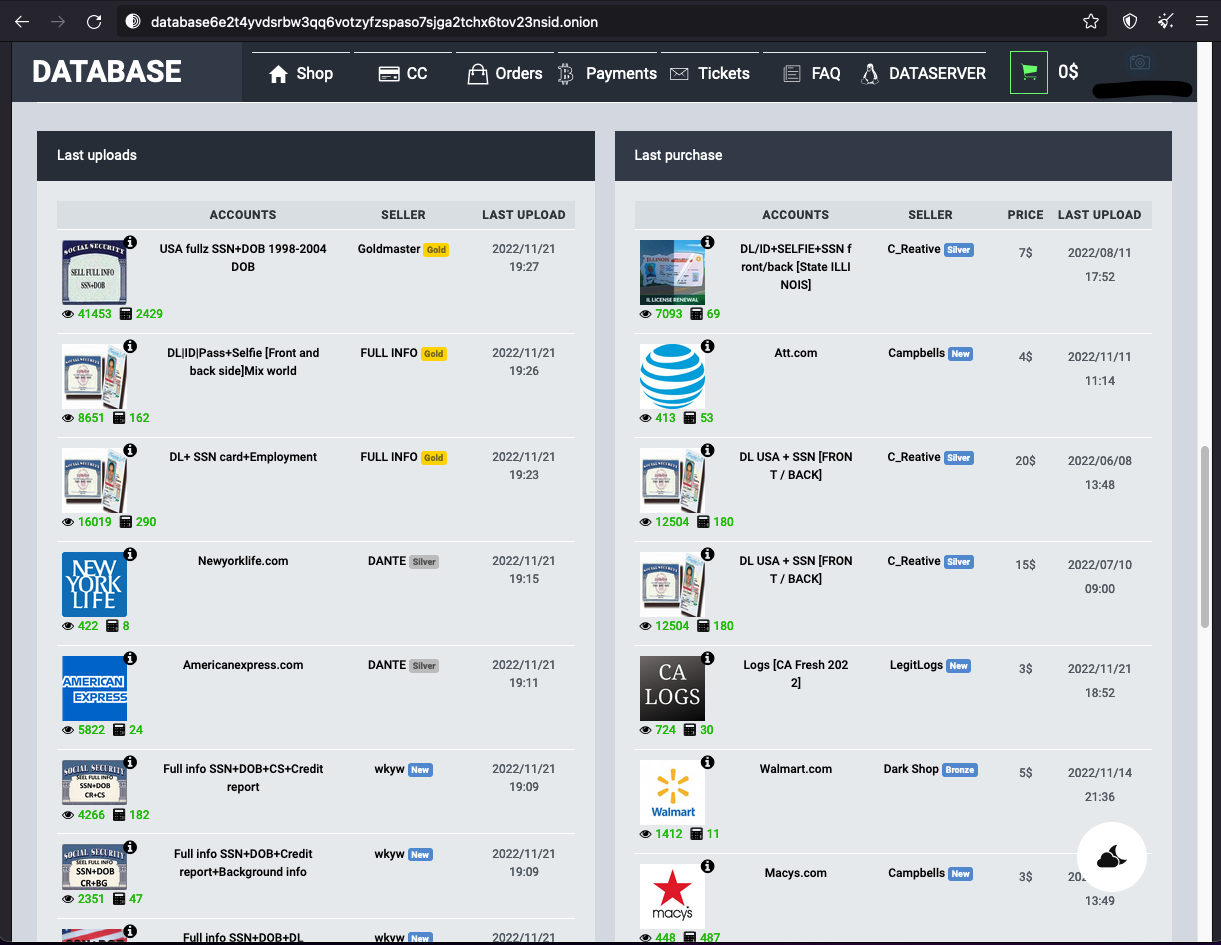
\includegraphics[width=\textwidth,height=\textheight,keepaspectratio]
    {screenshots/database_market_onion_service.png}
    \caption{Homepage of Database marketplace onion service hosted on Tor network.}
    \label{fig:database_homepage}
\end{figure}